\chapter{The Standard Model}
\label{chap:I-1-standard-model}

  The standard model provides a classification and description of the subatomic particles that compose our universe and their interactions. It describes both the particles of matter called fermions, which are subdivied among quarks and leptons, and the force carriers called bosons. Figure \ref{fig:I-1-sm-particles} gives a schematic view of the particle content of the standard model. Quarks and leptons are further divided into three generations with identical properties but increasing mass from which the first generation constitutes the everyday matter. Fermions interact with each other through the exchange of bosons. Gluons are the carriers of the strong force and interract solely with themselves and quarks as described by QCD. The photon, responsable for electromagnetism couples to all charged particles while the $ W^\pm $ and $ Z $ bosons couple to all particles except gluons as described by EWK. Finally, the Higgs boson as previously stated is the manifestation of the Higgs mechanism at the origin of mass. \\

	\begin{figure}[h!]
		\centering
		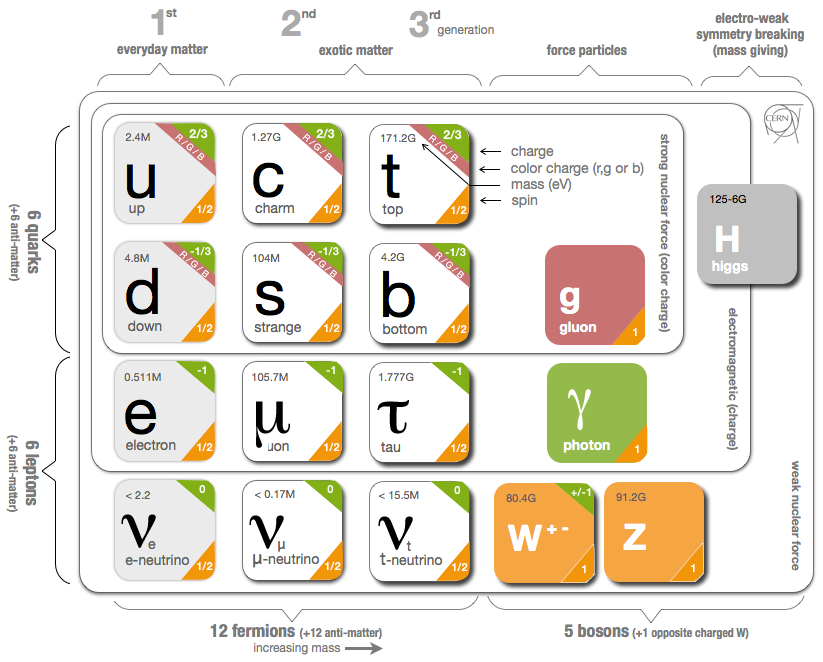
\includegraphics[width = 0.8 \textwidth]{img/I-1/sm-particles.png}
		\caption{Overview of the elementary particles as described by the standard model. Everyday matter is composed of the first generation of quarks and leptons to which two generations of heavier declinaisions are added. Gauge bosons or force particles are the carriers of the interactions between the other particles. The Higgs boson is the manifestation of the mechanism that gives mass to particles [CERN].}
		\label{fig:I-1-sm-particles}
	\end{figure}

  Besides classifying the particles, the standard model also provide as strong mathematical model built on top of quantum field theory and gauge invariance. The gauge group of the theory is $ SU(3)_C \otimes SU(2)_L \otimes U(1)_Y $, where $ SU(3)_C $ and $ SU(2)_L \otimes U(1)_Y $ are respectivly the symetry groups of the QCD and EWK sectors. Quarks and leptons are represented as fermionic fields within the lagrangian of the model while bosons arise from the invariance of the lagrangian under local gauge transformations.

  \section{Electroweak Theory}

    A local transformation of a fermionic field $ \psi $ under the gauge group of the EWK sector of the standard model $ SU(2)_L \otimes U(1)_Y $ can be written as

    \begin{equation}
      \psi \rightarrow \psi' = \exp\left( \frac{i}{2} g_W \Lambda^k(x) T^k \right) \exp\left( \frac{i}{2} g_W' \alpha(x) Y \right) \psi
    \end{equation}

    where $ g_W $, $ \Lambda^k(x) $, and $ T^k $ are respectivly the gauge coupling, local rotation parameters, and represenation of the $ SU(2)_L $ weak isospin algebra and $ g_W' $, $ \alpha(x) $, and $ Y $ their $ U(1)_Y $ counterparts. To preserve the invariance of the lagrangian

    \begin{equation}
      \mathcal{L} = i \bar{\psi} \gamma^\mu \partial_\mu \psi
    \end{equation}

    the partial derivate $ \partial_\mu $ must be rewriten as a covariant derivate

    \begin{equation}
      D_\mu = \partial_mu + i g_W W^k_\mu T^k + i g_W' B_\mu Y
    \end{equation}

    where $ W^k_\mu $ and $ B_\mu$ are the emerging gauge fiels associated to $ SU(2)_L $ and $ U(1)_Y $ required for the invariance of the theory.

  \section{Quantum Chromodynamics}

  \section{The Brout-Englert-Higgs Mechanism}

  \section{Beyond the Standard Model}
